\documentclass[12pt, a4paper]{report}

\usepackage[czech]{babel}
\usepackage[IL2]{fontenc}
\usepackage[utf8]{inputenc}
\usepackage{lmodern}  % lepší kvalita PDF

\usepackage[a4paper,top=3cm,bottom=3cm,left=3cm,right=3cm,marginparwidth=1.75cm]{geometry}

\usepackage{amsmath}
\usepackage{graphicx}
\usepackage{titling}
\usepackage{enumitem}
\usepackage[colorlinks=true, allcolors=black]{hyperref}
\usepackage{url}
\usepackage{caption}
\usepackage{subcaption}

% formátování zdrojového kódu
\usepackage{listings}
\usepackage{color}

\definecolor{dkgreen}{rgb}{0,0.6,0}
\definecolor{gray}{rgb}{0.5,0.5,0.5}
\definecolor{mauve}{rgb}{0.58,0,0.82}

\lstset{frame=tb,
	language=Java,
	aboveskip=3mm,
	belowskip=3mm,
	showstringspaces=false,
	columns=flexible,
	basicstyle={\small\ttfamily},
	numbers=none,
	numberstyle=\tiny\color{gray},
	keywordstyle=\color{blue},
	commentstyle=\color{dkgreen},
	stringstyle=\color{mauve},
	breaklines=true,
	breakatwhitespace=true,
	tabsize=4,
	extendedchars=true,
	literate=%
		{á}{{\'a}}1
		{č}{{\v{c}}}1
		{ď}{{\v{d}}}1
		{é}{{\'e}}1
		{ě}{{\v{e}}}1
		{í}{{\'i}}1
		{ň}{{\v{n}}}1
		{ó}{{\'o}}1
		{ř}{{\v{r}}}1
		{š}{{\v{s}}}1
		{ť}{{\v{t}}}1
		{ú}{{\'u}}1
		{ů}{{\r{u}}}1
		{ý}{{\'y}}1
		{ž}{{\v{z}}}1
		{Á}{{\'A}}1
		{Č}{{\v{C}}}1
		{Ď}{{\v{D}}}1
		{É}{{\'E}}1
		{Ě}{{\v{E}}}1
		{Í}{{\'I}}1
		{Ň}{{\v{N}}}1
		{Ó}{{\'O}}1
		{Ř}{{\v{R}}}1
		{Š}{{\v{S}}}1
		{Ť}{{\v{T}}}1
		{Ú}{{\'U}}1
		{Ů}{{\r{U}}}1
		{Ý}{{\'Y}}1
		{Ž}{{\v{Z}}}1
}
\lstset{language=Java}

\title{Vykreslování stromů}
\def \thesubtitle {Semestrální práce z předmětu KIV/PRO}
\author{Patrik Harag}
\def \theauthoremail {harag@students.zcu.cz}
\def \theauthorid {(A15B0034P)}

\begin{document}

\begin{titlepage}
	\begin{figure}
		
\includegraphics[height=50mm]{img-fav-logo}
	\end{figure}
	
	\centering
	{\large \hspace{1mm} \par} % tady musí být nějaký text jinak nefunguje vertikální odsazení
	\vspace{15ex}
	
	{\scshape\Large \thesubtitle \par}
	\vspace{1.5ex}
	{\huge\bfseries \thetitle \par}
	\vspace{2ex}
	{\Large\itshape \theauthor \par}
	\vspace{2ex}
	{\texttt{\theauthoremail} \par}
	\vspace{1ex}
	{\texttt{\theauthorid} \par}
	
	\vfill

	{\large \today\par}
\end{titlepage}

% strana s obsahem
\setcounter{page}{0} 
\tableofcontents
\thispagestyle{empty}

\chapter{Zadání}
Mnoho aplikací vyžaduje vykreslování obrázků stromů. Stromové diagramy jsou běžně používané pro vizualizaci adresářových struktur, rodokmenů nebo třeba abstraktních syntaktických stromů. Rozlišují se dva základní druhy stromů:
\begin{itemize}
	\item \emph{Zakořeněný strom} představuje hierarchii vycházející z jediného vrcholu nazývaného kořen. Diagram by měl reflektovat tuto hierarchii včetně pořadí, ve kterém se vyskytují jednotlivé vrcholy.
	Například rodokmeny jsou zakořeněné stromy a vrcholy představující sourozence jsou vykreslovány zleva doprava podle data narození.
	\item \emph{Volný strom} nemá žádný kořen ani hierarchickou strukturu. K vykreslování se tedy přistupuje zcela odlišným způsobem.
\end{itemize}
V této práci se budeme zabývat výhradně vykreslováním zakořeněných stromů.

\subsubsection*{Vstup}
Strom \emph{T}, jenž je grafem bez cyklů.
Rozměry vrcholů se neuvažují.

\subsubsection*{Výstup}
Hezký obrázek stromu \emph{T}.

\begin{figure}[ph]
	\centering
	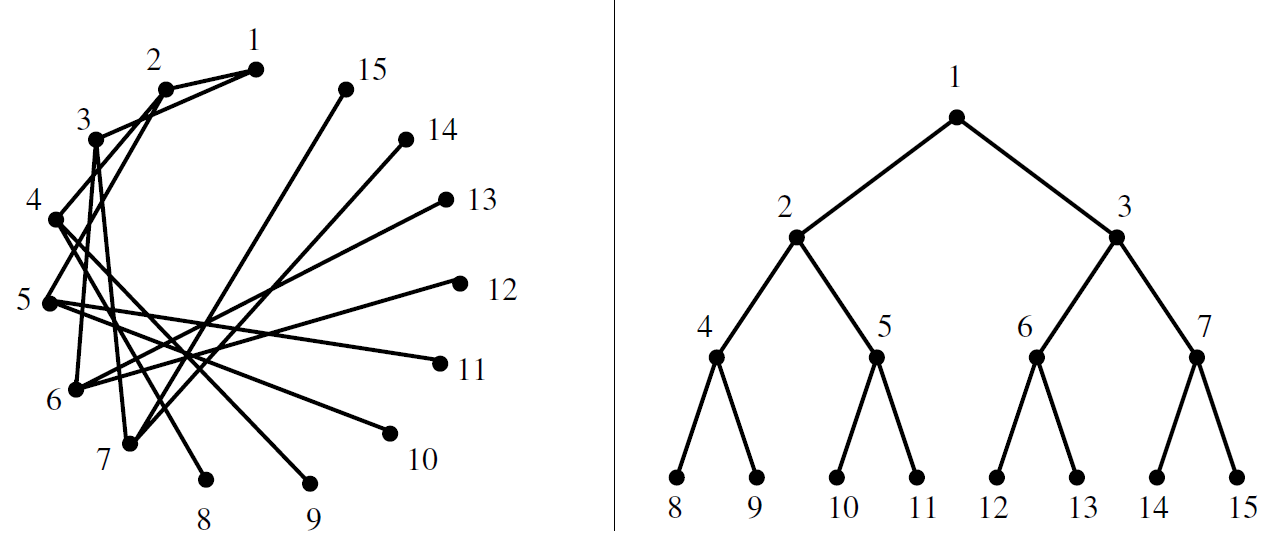
\includegraphics[width=0.8\linewidth]{img-io-example}
	\caption{Příklad vstupu a výstupu. Zdroj: \cite{Skiena09}}
	\label{fig:io-example}
\end{figure}

\chapter{Existující metody}
Existují dva základní způsoby vizualizace zakořeněných stromů:
\begin{itemize}
	\item \emph{Hierarchické rozložení} -- kořen je umístěn do středu horního okraje obrázku, strom roste směrem dolů. Alternativně může strom růst odspoda nahoru nebo z jedné boční strany na druhou.
	\item \emph{Středové rozložení} -- kořen je umístěn do středu obrázku, strom roste všemi směry. Toto rozložení je prostorově úspornější.
\end{itemize}
Výběr záleží především na konkrétní aplikaci. My se ale budeme zabývat výhradně standardním hierarchickým rozložením.

\section{Jednoduchý rekurzivní algoritmus}
\label{sec:simple-layout}
\begin{figure}
	\centering
	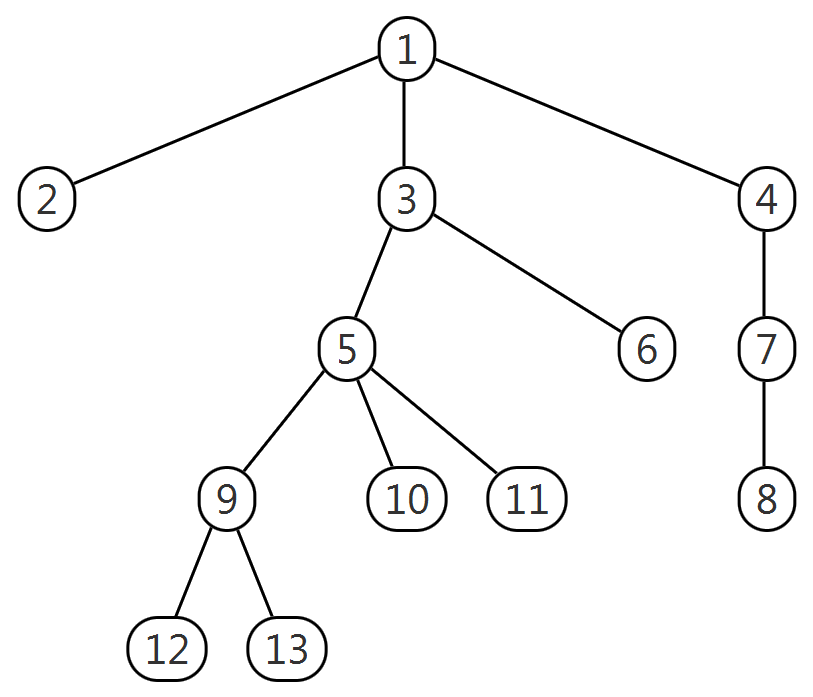
\includegraphics[height=0.5\linewidth]{img-simple-layout}
	\caption{Příklad stromu nakresleného jednoduchým rozmísťovacím algoritmem. Nevýhody tohoto algoritmu jsou jasně viditelné.}
	\label{fig:simple-layout}
\end{figure}

Algoritmus umístí kořen doprostřed horního okraje obrázku a obrázek vertikálně rozdělí na $n$ částí, kde $n$ je počet podstromů. Podstromy se rekurzivně vykreslí. Kořen podstromu je vždy umístěn do středu šířky, kterou zabírá celý jeho podstrom.

Ovšem tento algoritmus může vytvořit rozsáhlé prázdné plochy, jak je vidět na Obrázku \ref{fig:simple-layout}. To je dáno skutečností, že jsou sousední podstromy vykresleny vždy vedle sebe v pomyslném obdélníku a nemohou do sebe navzájem zasahovat. Tento problém nevznikne u vyvážených stromů, jako je například strom na Obrázku \ref{fig:io-example}.

\section{Reingold-Tilfordův algoritmu}
Reingold-Tilfordův algoritmus v podobě, v jaké byl představen \cite{reingold_tilford}, byl původně určen především k vykreslování binárních stromů. Nicméně je možné ho zobecnit, aby fungoval pro libovolný n-nární strom. 

Algoritmus spočívá v rekurzivní stavbě stromu odspoda. Jednotlivé podstromy se přiblíží a následně se nad ně vloží rodič zarovnaný na střed. Podstromy se takto postupně budují, dokud nedojde k vytvoření celého stromu.

Důležité vlastnosti tohoto algoritmu jsou, že se snaží strom vykreslit s co nejmenší šířkou a zachovává symetričnost. Pracuje v lineárním čase.

\section{Walkerův algoritmus}
Walkerův algoritmus \cite{walker} vychází z Reingold-Tilfordova algoritmu, ale zobecňuje jej pro použití na n-nárních stromech.

Algoritmus je dvouprůchodový. V prvním průchodu metodou \emph{postorder} jsou každému vrcholu přiřazeny dočasné souřadnice na ose $x$. V druhém průchodu metodou \emph{preorder} jsou tyto souřadnice ještě přepočítány.

Walkerův algoritmus byl později vylepšen, aby pracoval v lineárním čase \cite{buchheim}.

\chapter{Navržené řešení}
\label{sec:solution}

\section{Základní algoritmus}
Rozhodl jsem se navrhnout své vlastní řešení. Algoritmus funguje tak, že prochází strom metodou \emph{postorder} a přitom určuje pozice jednotlivých vrcholů i celých podstromů.

Každý podstrom je nejprve sestaven samostatně a pro každou jeho úroveň jsou určeny levé a pravé okraje. Jak jsou po sobě, zleva doprava, vytvářeny jednotlivé větve podstromu, je na základě levých okrajů všech jeho úrovní určena minimální velikost, o kolik se musí větev posunout směrem doprava. Poté se všechny vrcholy o tuto velikost posunou a dojde k přepočítání okrajů podstromu. Když jsou všechny větve podstromu zpracovány, zarovná se nad nimi jejich předek.

\section{Vylepšený algoritmus}
Výkon algoritmu popsaného výše kazí skutečnost, že je nutné opakovaně posouvat celé podstromy. U větších stromů by to mělo výrazný vliv na výkon.

Řešením je neposouvat celý podstrom ihned, ale jen uložit velikost posunutí do kořenu podstromu. Po dokončení standardního průchodu se celý strom projde ještě jednou a velikost posunutí se pro každý vrchol agreguje. 

\vfill

\subsection{Pseudokód}
\begin{lstlisting}
void make(tree) {
    makeSubtree(tree.getRoot(), 0);
    finalizeMove(tree.getRoot(), 0);
}

Bounds makeSubtree(node, level) {
    if (node nemá potomky) {
        nastavit node.x = 0, node.y = level * verticalSize 
        return okraje vrcholu
        
    } else {
        bounds = struktura pro uložení okrajů tohoto podstromu
        for (následníci n vrcholu node) {
            branch_bounds = makeSubtree(n, level + 1);
            výpočet velikosti posunu větve n směrem doprava na základě bounds a branch_bounds
            nastavení informace o posunutí n
            přepočítání okrajů podstromu (bounds)
        }
        
        nastavit node.x = vycentrování node nad jeho potomky,
                  node.y = level * verticalSize 
        
        přidání okrajů node do bounds
        return bounds
    }
}

void finalizeMove(node, totalOffset) {
    totalOffset += node.offset

    for (následníci n vrcholu node) {
        n.x += totalOffset;
        finalizeMove(n, totalOffset);
    }
}
\end{lstlisting}

\chapter{Experimenty a výsledky}
Program byl napsán v jazyce Java, verze 8. Pro uživatelské rozhraní a vykreslování byl použit framework JavaFX.

\section{Grafické výsledky}
Jak ukazuje Obrázek \ref{fig:compare-2}, algoritmus netrpí problémem s prázdnými plochami a jeho výstup má minimální šířku. Zároveň dodržuje hierarchii a pořadí vrcholů. Vykreslení rozsáhlejšího stromu ukazuje Obrázek \ref{fig:my-layout-large}.

\begin{figure}[ph]
	\centering
	\begin{subfigure}{0.5\textwidth}
		\centering
		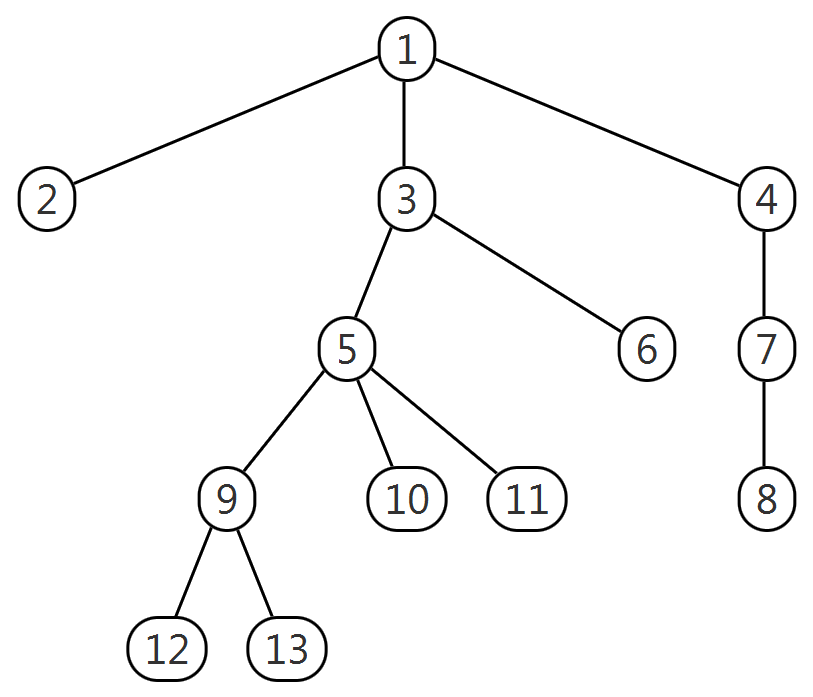
\includegraphics[height=0.8\linewidth]{img-simple-layout}
		\caption{Výstup algoritmu z kapitoly \ref{sec:simple-layout}.}
		\label{fig:compare-1}
	\end{subfigure}%
	\begin{subfigure}{0.5\textwidth}
		\centering
		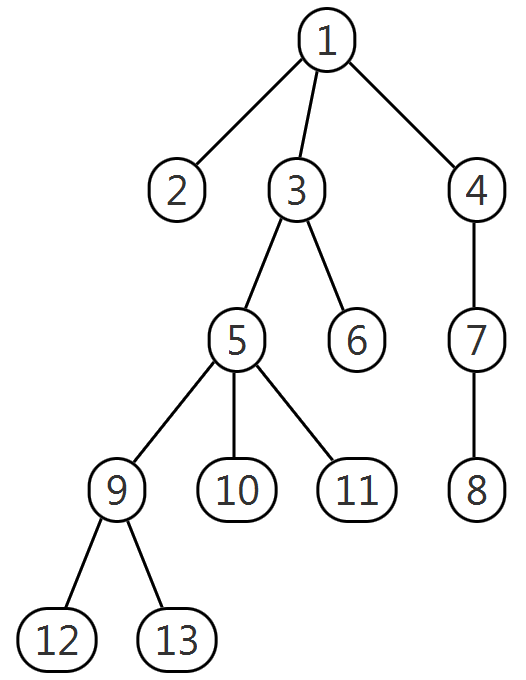
\includegraphics[height=0.8\linewidth]{img-my-layout}
		\caption{Výstup vlastního řešení.}
		\label{fig:compare-2}
	\end{subfigure}
	\caption{Porovnání výstupu jednoduchého algoritmu a vlastního řešení.}
	\label{fig:compare}
\end{figure}

\begin{figure}
	\centering
	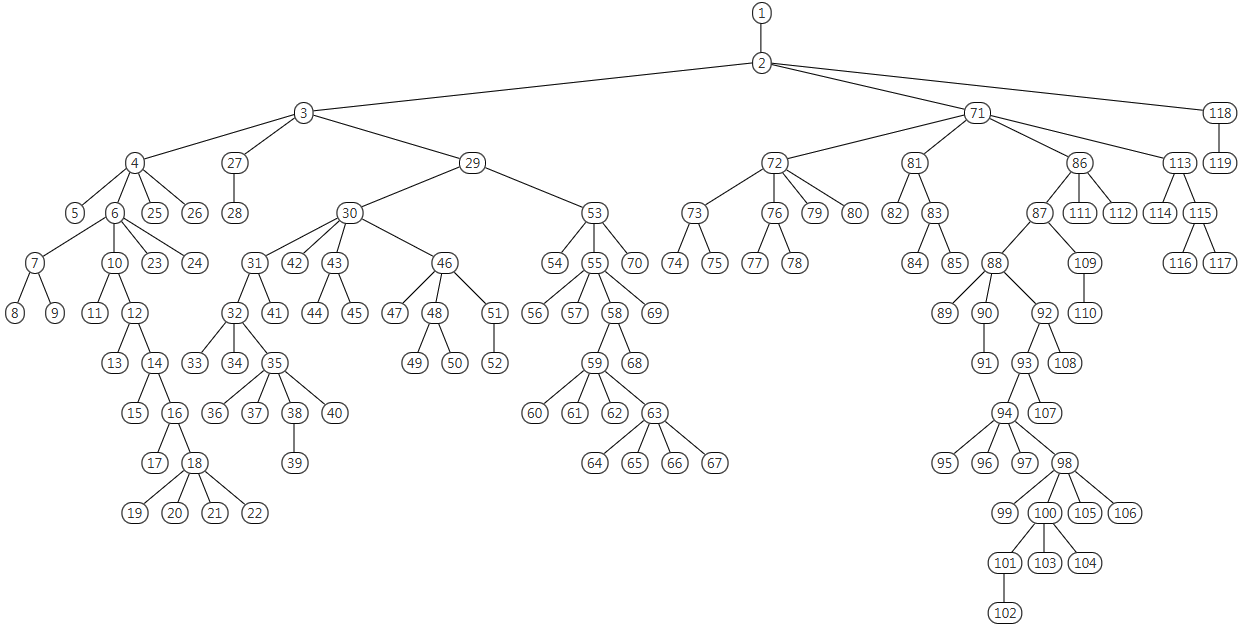
\includegraphics[width=1\linewidth]{img-my-layout-large}
	\caption{Vykreslení rozsáhlejšího stromu.}
	\label{fig:my-layout-large}
\end{figure}

\section{Měření rychlosti}
Pro měření rychlosti byly vygenerovány náhodné stromy o nastaveném maximálním počtu až 9 následníků a maximální hloubce až 30 úrovní. Měření zahrnovalo pouze běh pozicovacího algoritmu, nikoli samotné vykreslování.
Bodle Tabulky \ref{tbl:performance} se dá říci, že rychlost algoritmu určitě nebude při jeho běžném použití překážkou.

\begin{table}
	\caption{Doby běhů jednotlivých algoritmů na procesoru Intel Core i5-4570. Hodnoty jsou zaokrouhleny na celá čísla, počty vrcholů na tisíce.}
	\centering
	\label{tbl:performance}
	\begin{tabular}{l|llll}
		Počet vrcholů & Jednoduchý alg. & Vlastní alg. & Vlastní alg. (vylepšený) \\
		 \hline
		3 000 & 0 ns & 1 ns & 1 ns \\
		10 000 & 0 ns & 8 ns & 7 ns \\
		45 000 & 2 ns & 24 ns & 24 ns \\
		125 000 & 5 ns & 65 ns & 37 ns \\
		270 000 & 7 ns & 122 ns & 77 ns \\
		2 050 000 & 50 ns & 902 ns & 408 ns \\
	\end{tabular}
\end{table}


\chapter{Závěr}
Navrhli a implementovali jsme algoritmus pro kreslení obecných n-nárních stromů, který dává dobrý grafický výstup a je dostatečně efektivní na to, aby mohl být použit i v praxi.

V rámci experimentů byla vytvořena jednoduchá aplikace v JavaFX, která dokáže vykreslit stromy nejen navrženým algoritmem popsaném v kapitole \ref{sec:solution}, ale i jednoduchým rekurzivním algoritmem z kapitoly \ref{sec:simple-layout}. Všechny obrázky použité v této práci od kapitoly 2 byly vykresleny touto aplikací.

\bibliographystyle{alphaurl}
\bibliography{sources}

\end{document}